% !TeX program = xelatex
\documentclass{article}

% ------- Packages and Settings --------
 
% GENERAL 

%
% Load KNMI poster package
%
% 	Options:
%
%	portrait* | landscape		set poster orientation
%	cmyk* | rgb		 	set pdf colour mode
% 	english* | dutch			set KNMI logo language
% 	epslogo* | pdflogo		set KNMI logo format
% 	disablefonts			disable all custom fonts (and the need for XeLaTeX)
% 	path			 		specify path to ?KNMIposter? (default = current directory)
% 	fixfooter			 	fix footer spacing (required for some Tex/Postscript versions)
% 	debug			 	enable geometry showframe
%
% * = default
%
\usepackage[landscape]{KNMIposter}


% USER PACKAGES
% language
\usepackage[english]{babel}

% Define path for figures -- for safety, keep the last /
\graphicspath{{example_figures/}}

% Assist LaTeX in hyphenation
\hyphenation{Rey-nold}
\hyphenation{Ra-ma-swa-my}


% USER PACKAGES
% language
\usepackage[english]{babel}

% Define path for figures -- for safety, keep the last /
\graphicspath{{EGU_figures/}}

% Assist LaTeX in hyphenation
\hyphenation{Rey-nold}
\hyphenation{Ra-ma-swa-my}



% ------- POSTER HEADER --------

% Poster title
\title{Automatic fog detection for public safety by using camera images}

% Author
\author{Giuliano Andrea Pagani\affil{1}, Martin Roth\affil{1}, and Wiel Wauben\affil{1}. Contact: \email{pagani@knmi.nl}}

% Affiliations
\affiliations{\affil{1}R\&D Department of Observations and Data-Technology, Royal Netherlands Meteorological Institute. PO Box 201, 3730 AE De Bilt, The Netherlands.%
}

% You can either add the contact information in the author line (poster top, large),
% or in the affiliations (poster bottom, footnote size).

% Some additional space for acknowledgements, url's, ... 
% \acknowledge{I would like to thank all of you!}


% ------- Document start --------
\begin{document}

\maketitle

\begin{abstract}
Visibility is traditionally measured manually by meteorological observers using landmarks at known distances in
the vicinity of the observation site. 
%Nowadays, distributed cameras facilitate inspection of more locations from one
%remote monitoring center. The main idea is, however, still deriving the visibility or presence of fog by an operator
%judging the scenery and the presence of landmarks. 
Visibility sensors are also used, but they are rather costly and
require regular maintenance. Moreover, observers, and in particular sensors, give only visibility information that is
representative for a limited area. 
Cameras are more and more deployed for surveillance and security reasons in cities and for monitoring traffic along
main transportation ways. In addition to this primary use of cameras, we consider cameras as potential sensors to
automatically identify low visibility conditions. 
The approach that we follow is to use machine learning techniques
to determine the presence of fog and/or to make an estimation of the visibility. 
%For that purpose a set of features
%are extracted from the camera images such as the number of edges, brightness, transmission of the image dark
%channel, fractal dimension. In addition to these image features, we also consider meteorological variables such
%as wind speed, temperature, relative humidity, and dew point as additional features to feed the machine learning
%model. %Furthermore, it is shown how to generate a pdf file which can easily be handled by the studio for printing.
\end{abstract}

\bcols %% Start columns

\section*{Motivation}
Fog and reduced visibility have considerable impact on the performance of road, maritime, and aeronautical transportation
networks. The impact ranges from minor delays to more serious congestions or unavailability of the
infrastructure and can even lead to damage or loss of lives~\cite{gultepe07}.

%\vspace{-0.5cm}
\begin{minipage}[b]{\columnwidth}
	\begin{center}
	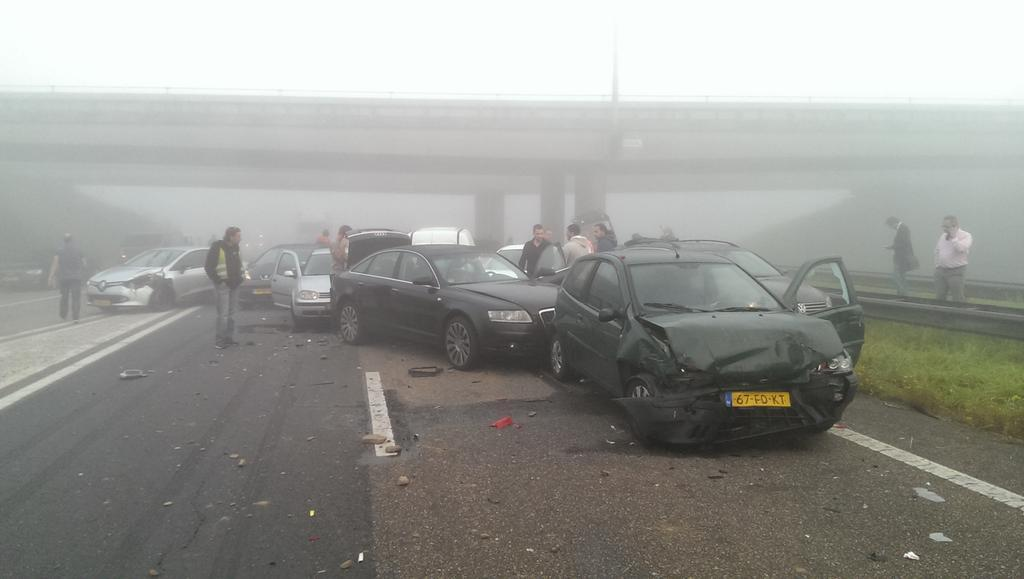
\includegraphics[width=0.9\columnwidth]{Accident}
	\captionof{figure}{Traffic accident caused by dense fog conditions.}
	\label{figAccident}
	\end{center}
\end{minipage}
\vspace{-2cm}

\subsection*{Key facts:}
\begin{itemize}
  \item May form and dissipate suddenly.
  \item Often only a local phenomenon.
\end{itemize}

\subsection*{Why current technology is not enough:}
\begin{itemize}
\item Satellites are not constantly observing areas of interest.
\item Weather stations observe a limited area.
\item Forecast of fog conditions is complex.
\end{itemize}

\subsection*{Idea:}
Use camera deployed for surveillance and security reasons in cities and for monitoring traffic along
main transportation ways as potential sensors to
automatically identify low visibility conditions.


\begin{minipage}[b]{\columnwidth}
\centering
\begin{minipage}[b]{0.4\columnwidth}
	\begin{center}
	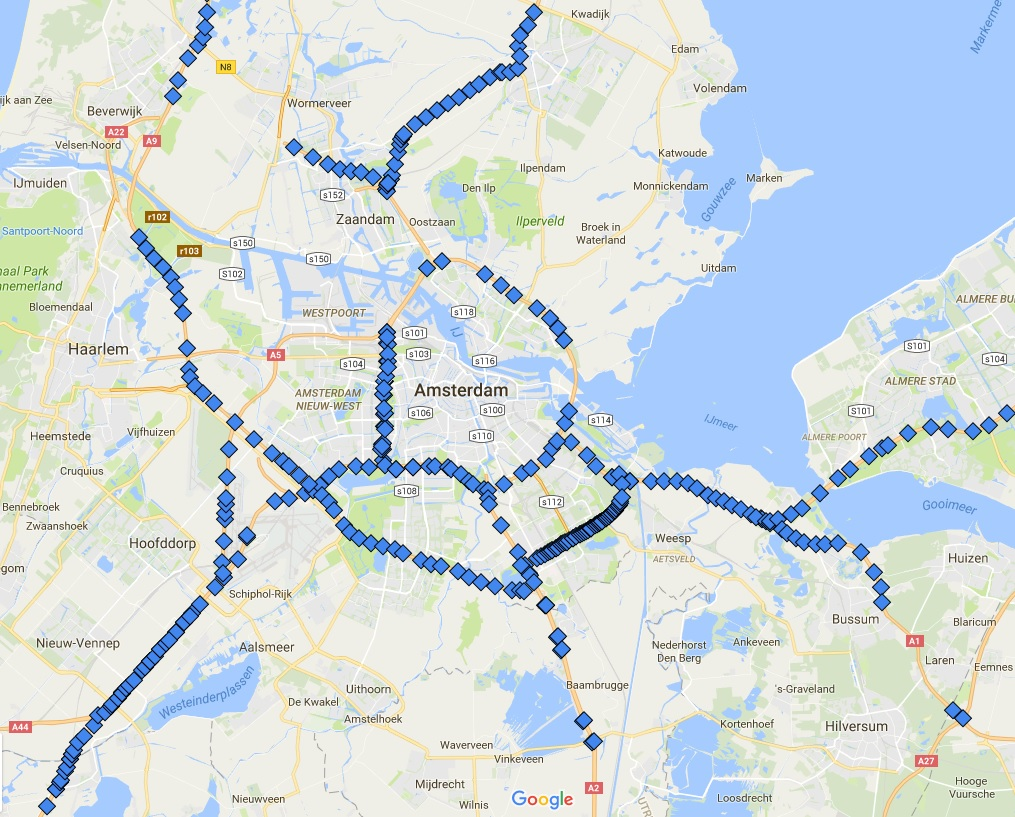
\includegraphics[width=\columnwidth]{CameraPlacement}
	\captionof{figure}{Cameras monitoring highways in Amsterdam region.}
	\label{figCameras}
	\end{center}
	\end{minipage}
	\hspace*{0.1cm}
\begin{minipage}[b]{0.4\columnwidth}
	\begin{center}
	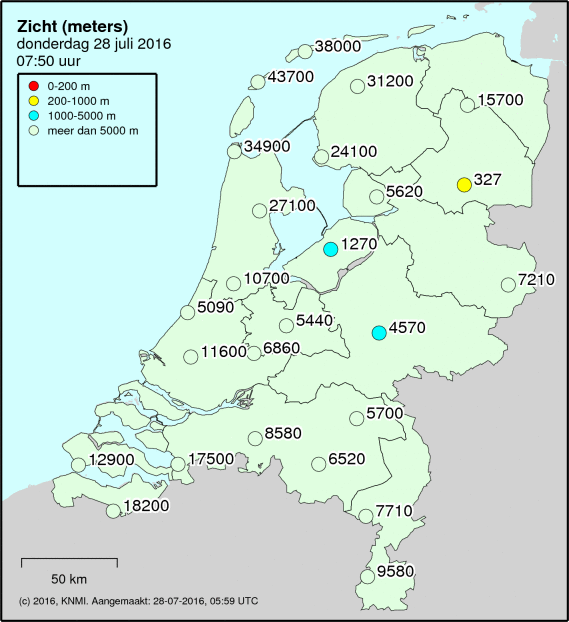
\includegraphics[width=\columnwidth]{SensorPlacement}
	\captionof{figure}{KNMI weather stations locations.}
	\label{figSensors}
	\end{center}
\end{minipage}
\end{minipage}

\section*{Approach}
\subsection*{From Pictures to Machine Learning}
Pictures are translated to a set of quantities capturing their properties (\textbf{features}).\newline
The meteorological transmissionmeter sensor provide ground truth for the visibility conditions in the measurement field (\textbf{supervised} problem).
\textit{Restrictions}: i) static cameras, ii) daylight conditions, iii) period: 3/2015 - present.

\subsection*{Features}
\begin{itemize}
\item{Image based:}
\begin{itemize}
\item{Mean Edges: for finding the boundaries of objects within images. It works by detecting discontinuities in the image (e.g., foreground and background elements).}
\item{Mean Brightness: perception of a source of radiating/reflecting light.}
\item{Mean Saturation: is a measure of the purity of the color. The purest (most saturated) color is achieved by using just one wavelength, less pure come from a combination at different wavelegths.}
\item{Mean HUE: perception of a source of being similar to one of the perceived colors: red, yellow, green, and blue, or to a combination of two of them.}
\item{Fractal Dimension: self similarity in filling space.}
\item{Transmission smoothness: transmission of the darkchannel of the image (smoothed indicator).}
\item{Transmission changepoint: horizontal point where the transmission of the dark channel is subject to change.}
\end{itemize}
\item{Weather info:}
\begin{itemize}
\item{Wind speed}
\item{Dew point}
\item{Humidity}
\item{Precipitation amount}
\end{itemize}
\end{itemize}


\begin{minipage}[b]{\columnwidth}
	\begin{center}
	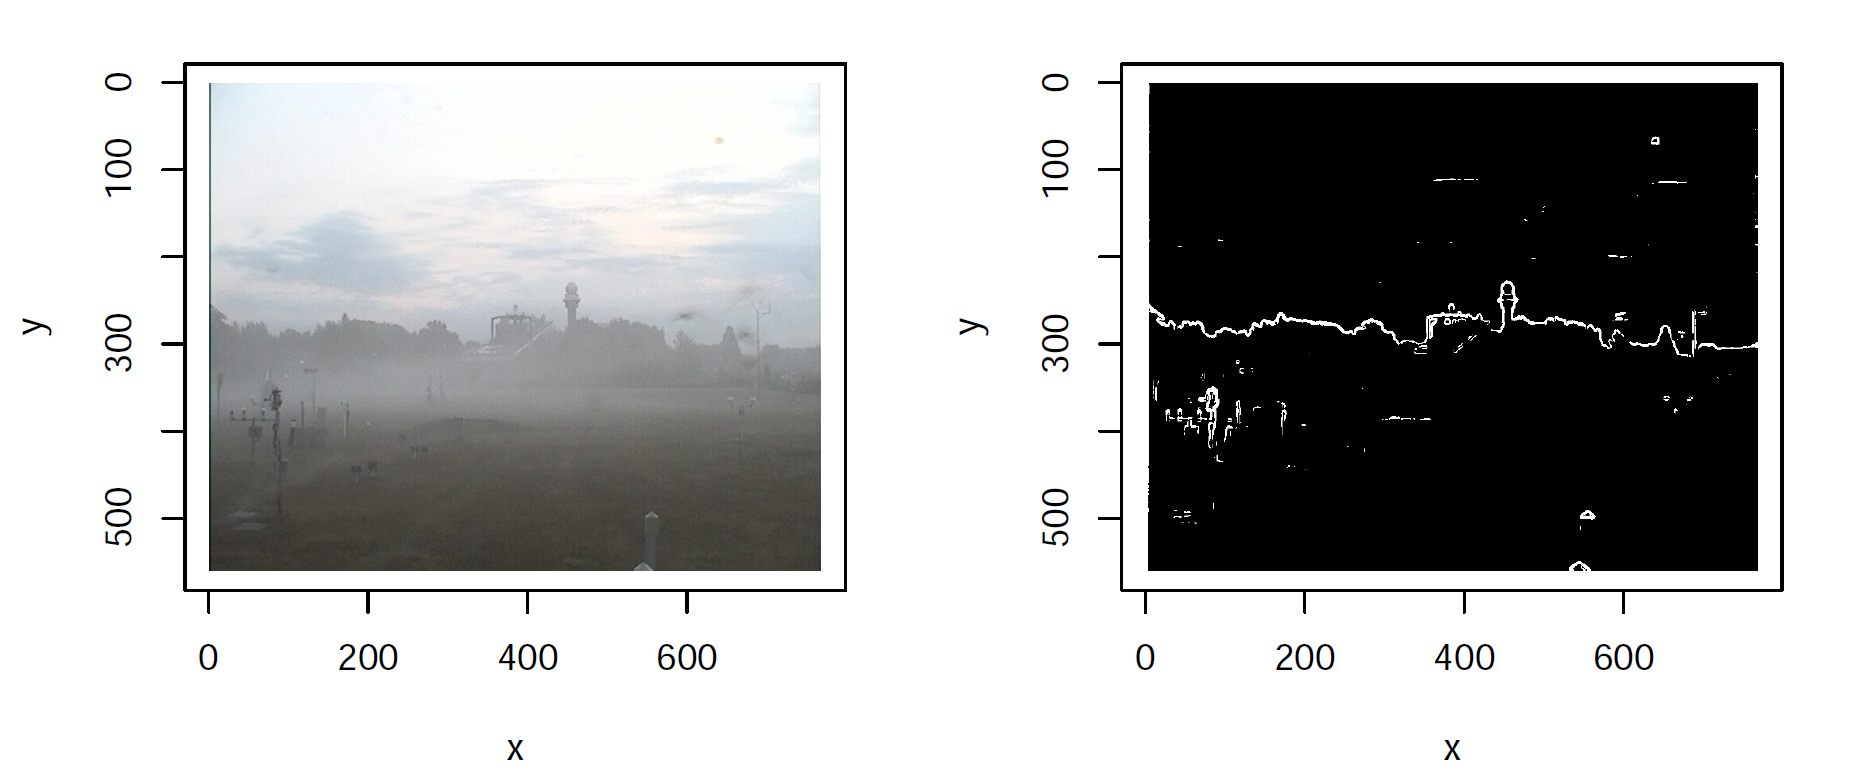
\includegraphics[width=0.95\columnwidth]{edges}
	\captionof{figure}{Edge detection.}
	\label{figEdges}
	\end{center}
\end{minipage}

\begin{minipage}[b]{\columnwidth}
	\begin{center}
	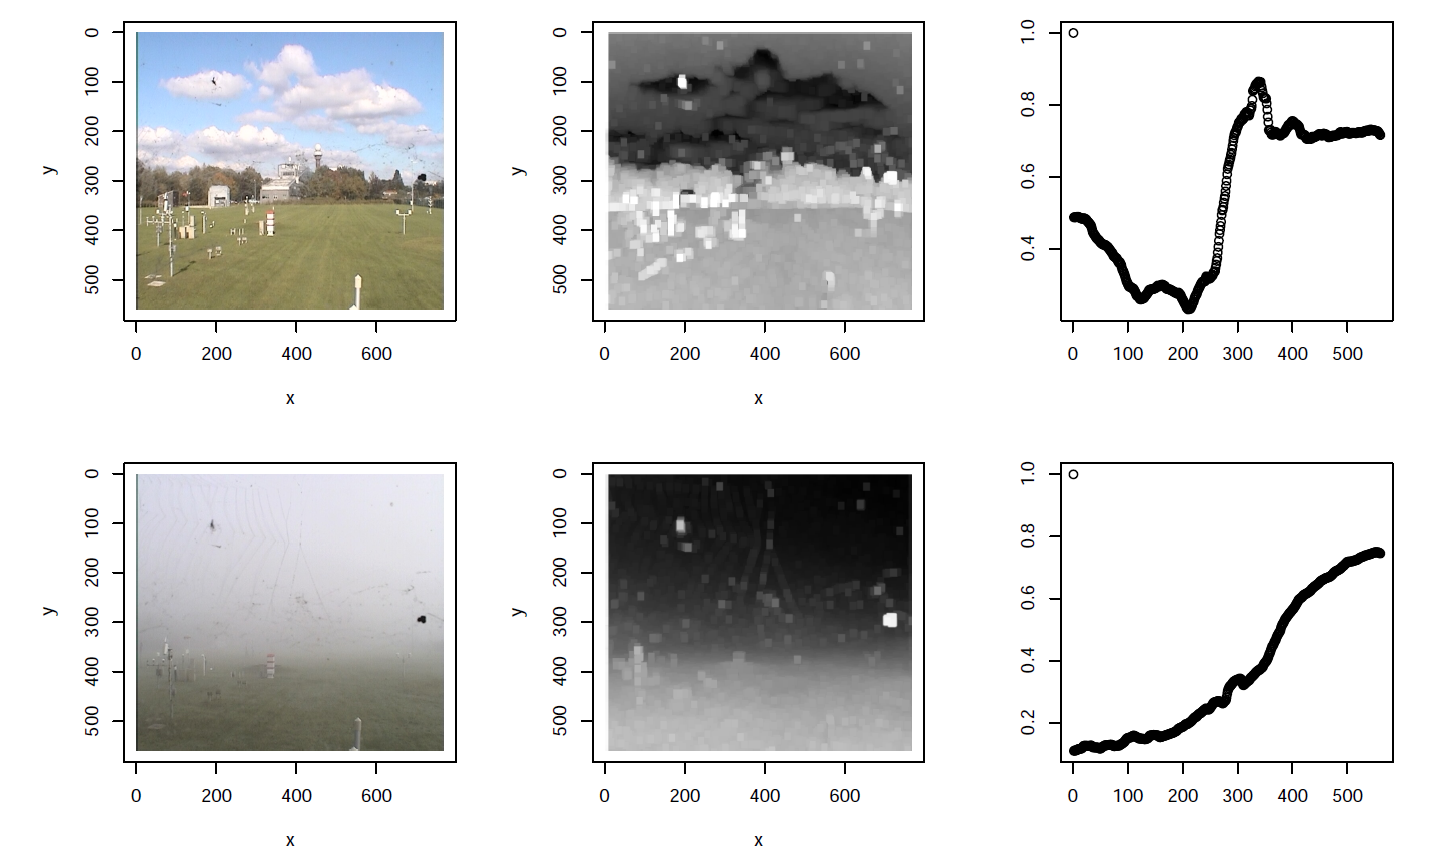
\includegraphics[width=0.95\columnwidth]{transmission}
	\captionof{figure}{Average horizontal dark channel transmission clear (top) and foggy (bottom) day.}
	\label{figTransmission}
	\end{center}
\end{minipage}





\subsection*{Sections and subsections}
Sections and subsections can be used both with numbering (e.g., \verb|\section|) or without numbering (e.g.,\verb|\section*|).

\subsection*{Typesetting}
Font and typesetting are included in the package for A0 posters. Just make use of the default \latex commands. Need to change the text-size?
{\tiny tiny}, 
{\scriptsize scriptsize}, 
{\footnotesize footnotesize}, 
{\small small}, 
{\normalsize normalsize}, 
{\large large}, 
{\Large Large}, 
{\LARGE LARGE},
{\huge huge}, 
{\Huge Huge}.
Or set other styles like \textit{italic}, \textbf{bold}, \underline{underline}, \textsc{small caps}.

\pushdown % similar to vfil (=vfill, but fixed for the column floats)

% Figure exactly 2 columns width
% \vspace{20pt plus 10pt minus 5pt}
% \begin{minipage}[b]{\twocolwidth}
% 	\begin{center}
% 	\includegraphics[width=\twocolwidth]{fig3}
% 	\captionof{figure}{A figure spanning two columns.}
% 	\label{2col-fig}
% 	\end{center}
% \end{minipage}

\columnbreak % force jump to next column

\section*{Results}
Figures and tables need to be placed within a \verb|minipage| environment to keep all elements together and enable easy positioning.
However, leave out the default \latex wrapper environments \verb|figure| and \verb|table| as floats are messed up in the column environment.

\subsection*{Figures}

Preferred figure formats are vectors (e.g., PDF or EPS) for proper color handling (cmyk) and scaling when printing. It is best to size the figure by relative scaling with respect to the column width, e.g., \verb|width=1.0\columnwidth|.
Captions are added to figures by appending \verb|\captionof{figure}{...}| after the \verb|\includegraphics| line. Figures \ref{fig1} shows an example.

\subsection*{Tables}
Table \ref{table} demonstrates how tables can be added within a columns, or even spanning multiple ones. It only uses the \verb|tabular| environment. A caption can be added using \verb|\captionof{table}{...}|. 

\subsection*{Multi column figures and tables}
It is possible to make a figure and tables span multiple columns. If you need it as wide as the entire page, just place it outside the \verb|\bcols| and \verb|\ecols| commands. Need the full-page figure in the middle of the page? Just make \verb|\bcols| and \verb|\ecols| environments before and after it!

%%%%%%%%%%%
% Fix text overflow for two column figure !!!
%%%%%%%%%%%
\pushdown
\begin{minipage}[b]{\columnwidth}
\end{minipage}
%%%%%%%%%%%

\columnbreak

% Figure
\vspace{20pt plus 10pt minus 5pt}
% \begin{minipage}[b]{\columnwidth}
% 	\begin{center}
% 	\includegraphics[width=1.0\columnwidth]{fig1}
% 	\captionof{figure}{Imaginary part of the refractive index of ice and water as a function of wavelength.}
% 	\label{fig1}
% 	\end{center}
% \end{minipage}
\vspace{-1em}

Figure \ref{2col-fig} shows a two column figure. By making the \verb|minipage| two column wide, you extend the area to next column. However, floating and text overflow are not automated, so it is up to you to add a \verb|\columnbreak| and an empty \verb|minipage|.



\section*{Follow up - Open Questions?}
The compiled \latex document directly generates an A0 pdf. However, you do can directly print it out on a scaled paper format, for example, A4 or A3, using one of the colour printers.
To have the poster printed on full size (4 times A4, or A0) by the studio, is only a matter of providing them your compiled pdf.

% Table
\vspace{20pt plus 10pt minus 5pt}
\begin{minipage}[b]{\columnwidth}
%
\captionof{table}{A demonstration of how to add a table and caption to the poster, showing some waveform characteristics: trace velocity ($c_{\text{app}}$) and bearing deviation ($\Delta\phi$) compared individually as well as combined (all).}
\begin{center}
\begin{tabular}{l r r | r r | r r}
\hline
& \multicolumn{2}{c}{$c_{\text{app}}$} &  \multicolumn{2}{|c}{$\Delta\phi$} &  \multicolumn{2}{|c}{all} \\
\cline{2-7}
& \multicolumn{6}{c}{hits (percentage)} \\
\hline
Analysis 	& 93	&(26.0\%) & 76 & (21.2\%) &  22 & (6.1\%) \\
Ensemble & 183 &(51.1\%) & 151 & (42.2\%)  & 70 & (19.6\%) \\
%\hline
Score & +90 & (+96.8\%) & +75 & (+98.7\%)  & +48 & (+218.2\%) \\
\hline
\end{tabular}
\end{center}
\label{table}
%
\end{minipage}


% Figure
% \vspace{20pt plus 10pt minus 5pt}
% \begin{minipage}[b]{\columnwidth}\begin{center}
% 	\begin{center}
% 	\includegraphics[width=\columnwidth]{fig2}
% 	\captionof{figure}{Part of an AVIRIS flight line acquired over the Pacific Ocean. Left half: a water cloud (Sc), right half: an ice cloud (Ci).}
% 	\label{fig2}
% 	\end{center}
% \end{center}\end{minipage}

\section*{Conclusion}
This standard poster offers the possibility of using \latex for making a KNMI-style poster. The procedure is simple because the layout of the poster is contained within this document. It is suggested not to change the layout, but you are free to tweak the \latex code within the defined page area to fit your needs. Bugs and questions related to this \latex style package? Contact Pieter Smets, \email{smets@knmi.nl}, room A3.06.

\pushdown

\begin{fminipage}{\columnwidth}
\textit{%
\noindent This is an edition from the KNMI in \\
cooperation with
} %
% \begin{center}\includegraphics[width=.7\columnwidth,clip,trim=0 .4cm 0 .2cm]{TU}\end{center}%
\end{fminipage}

\ecols %% End columns 

\end{document}
